%\chapter{Extraction de quantités thermodynamiques des images expérimentales}
\chapter{Traitement des images expérimentales}
\label{ch:anex_mesure_temp}

\section{Détermination du profil de densité intégrée}

Les images expérimentales obtenues correspondent à des profils de densité intégrés suivant l'axe d'imagerie, il s'agit de profils de densité bidimensionnels $n_{\mathrm{2D}}(y,z)$ (pour une imagerie selon l'axe $\vec{x}$).

Pour faciliter le traitement des images expérimentales, on détermine un profil unidimensionnel à l'aide d'une intégration suivant une seconde direction. On obtient ainsi un profil $n_{\mathrm{1D}}$: 
\begin{equation}
n_{\mathrm{1D}}(z)=\int{\diff y \: n_{\mathrm{2D}}(y,z)} \text{ ,}
\end{equation}
sur lequel nous effectuons nos opérations de détermination des grandeurs thermodynamiques.

Dans le cas de nuages thermiques, ces profils unidimensionnels sont ajustés à l'aide d'une gaussienne, dont l'intégrale fournit le nombre d'atomes présent dans le nuage, le centre fournit la position du nuage suivant la direction considérée, et enfin la largeur nous donne une mesure de la taille du nuage suivant cette même direction.















\section{Estimation de la température}
\subsection{Mesure de la température par temps de vol}
De manière générale, la température du gaz est estimée à l'aide d'une imagerie par \emph{temps de vol}. Son principe repose sur l'expansion libre du nuage après extinction du piège, expansion dont l'origine provient de la distribution des vitesses des atomes. Dans le cas d'un nuage thermique, la température est donnée par la largeur de la distribution des vitesses du gaz, qui est directement donnée par la taille du nuage après un temps d'expansion suffisamment long.

La taille d'un nuage thermique évolue suivant la direction $\vec{i}$ selon
\begin{equation}
\sigma_{\mathrm{i}}^2(t)= \sigma_{\mathrm{i,0}}^2+ t^2 \kB T/m \text{ ,}
\end{equation}
avec $T$ la température du nuage, $m$ la masse des atomes, $t$ le temps d'expansion après extinction du piège, et $\sigma_{\mathrm{i,0}}=\sigma_{\mathrm{i}}(t=0)$ la taille initiale du nuage piégé. Notons que cette expression n'est valable que dans le cas d'un nuage dilué, pour lequel les interactions peuvent être négligées.

Pour des temps d'expansion $t$ suffisamment grands, tels que le déplacement des atomes durant la phase d'expansion soit très grand devant la taille initiale du nuage, il est ainsi possible de négliger cette dernière. La taille mesurée du nuage donne alors directement accès à sa température.





\subsection{Estimation de la température d'un nuage lévité}
Cependant, pour des nuages particulièrement froids, les temps d'expansion requis pour estimer correctement la température du nuage peuvent dépasser le temps d'observation possible des atomes alors en mouvement de chute libre. L'utilisation de la lévitation magnétique pendant cette phase d'expansion permet de dépasser cette limite en compensant la gravité\footnote{La pesanteur a pour effet de \textit{pencher} le potentiel, pouvant changer la dimensionnalité de l'évaporation \citep{boyer2000condensation}, mais aussi limiter la profondeur du piège optique à environ $U/\kB \sim \SI{2.5}{\micro\kelvin}$ pour laquelle la gradient maximal d'intensité lumineuse ne permet plus de compenser le poids des atomes. L'utilisation de la lévitation magnétique au cours de l'évaporation permet alors de dépasser cette limitation. }, permettant aux atomes de rester plus longtemps dans la zone d'imagerie. Néanmoins, comme nous l'avons détaillé dans la section \ref{sc:oscillations_levitation}, l'utilisation de la lévitation magnétique conduit à un piégeage résiduel de l'état $\etatF{1}{-1}$ dans lequel nous souhaitons franchir le seuil de condensation.

L'estimation correcte de la température du nuage lévité repose alors sur deux contraintes que le temps d'expansion du nuage doit satisfaire: 
\begin{itemize}
\item[\textendash] Celui-ci doit être suffisamment grand pour pouvoir négliger la taille initiale du nuage devant celle mesurée.
\item[\textendash] Le temps d'expansion doit être suffisamment petit devant la période d'oscillation de la taille du nuage, liée au piégeage de la lévitation magnétique. De cette manière, l'expansion peut être considérée balistique.
\end{itemize}
Dans la configuration à bas champ de la lévitation magnétique, proche du biais magique $\magicB=\SI{3.2}{\gauss}$, les fréquences de piégeage sont particulièrement grandes et il n'est pas possible de satisfaire ces deux contraintes simultanément. 

La méthode retenue par l'équipe pour obtenir une mesure correcte de la température du nuage repose sur la technique de \emph{focalisation atomique}. Celle-ci permet d'imager dans l'espace réel la distribution de vitesses à l'aide d'un potentiel harmonique, à l'instar d'une lentille en optique \citep{murthy2014matter}. Pour illustrer ces propos, considérons un ensemble d'atomes dont la distribution initiale des positions est de largeur $\Delta\mathrm{x}_{\mathrm{i,0}}$ dans la direction $\vec{i}$ et la distribution de vitesses est de largeur $\Delta\mathrm{v}_{\mathrm{i,0}}=\hb \Delta\mathrm{k}_{\mathrm{i,0}} /m$. Sous l'effet du potentiel harmonique, l'évolution temporelle de la largeur de la distribution de positions est donnée par
\begin{equation}
\Delta\mathrm{x}_{\mathrm{i}}^2(t)=\Delta\mathrm{x}_{\mathrm{i,0}}^2 \cos^2(\omega_{\mathrm{i}} t) + \frac{\hb^2 \Delta\mathrm{k}_{\mathrm{i,0}}^2}{m^2 \omega_{\mathrm{i}}^2} \sin^2(\omega_{\mathrm{i}} t) \text{ ,}
\end{equation}
tel qu'illustré schématiquement figure \ref{fig:focalisation_atomique}.

En coupant le potentiel harmonique après un quart d'oscillation à $t=T_{\mathrm{osc}}/4$ avec $T_{\mathrm{osc}}= 2\pi/\omega_{\mathrm{i}}$ la période d'oscillation, la distribution de positions des atomes a une largeur donnée par
\begin{equation}
\Delta\mathrm{x}_{\mathrm{i}}(T_{\mathrm{osc}}/4)=\left|\frac{\hb \Delta\mathrm{k}_{\mathrm{i,0}}}{m \omega_{\mathrm{i}}}\right| \text{ ,}
\end{equation}
qui ne dépend que de la distribution initiale d'impulsion des atomes. À l'aide de la distribution thermique des vitesses, on déduit finalement que la température s'exprime
\begin{equation}
T=\frac{m \omega_{\mathrm{i}}^2 \Delta \mathrm{x}_{\mathrm{i}}^2(T_{\mathrm{osc}}/4)}{\kB} \text{ .}
\end{equation}

Cette mesure de la température est donc indépendante de la taille initiale du nuage, contrairement à la mesure par temps de vol qui nécessite une longue expansion pour s'affranchir de l'influence de la taille initiale. Une seconde différence entre ces méthodes réside dans le fait que le temps d'expansion par focalisation atomique n'est plus ajustable, celui-ci étant fixé par la fréquence du piégeage harmonique de la lévitation magnétique. 

De plus, notons que dans la configuration de faible champ magnétique choisie, le piégeage vertical est négligeable devant celui des directions horizontales. En considérant que l'expansion du nuage est balistique suivant la direction verticale, l'estimation de la température obtenue par temps de vol est en accord avec les valeurs extraites par focalisation atomique suivant les deux directions horizontales, comme illustré figure \ref{fig:focalisation_atomique}.b.

\begin{figure}
\centering
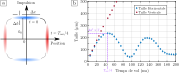
\includegraphics[width=\textwidth]{Fig/Modif_exp/focalisation_atomique.pdf}
\caption{\textbf{a: Principe de la focalisation atomique.} L'évolution temporelle d'un nuage dans l'espace des phases est une rotation autour de l'origine. À $t=T_{\mathrm{osc}}/4$, la distribution du nuage dans l'espace des phases a subi une rotation de $-\pi/2$. On peut ainsi mesurer la distribution initiale d'impulsion par une mesure de densité atomique dans l'espace réel. \textbf{b: Évolution temporelle de la taille du nuage dans la champ de lévitation.} Le piégeage étant quasi-nul dans la direction verticale, le nuage s'étend de manière balistique (points bordeaux). Dans la direction horizontale, le nuage subit l'effet de piégeage harmonique de la lévitation magnétique et sa taille oscille à une fréquence correspondant au double de la fréquence de piégeage (points bleus). Pour un temps de vol d'environ \SI{45}{\milli\second}, le nuage atteint sa taille maximale représentative de la distribution initiale d'impulsion. Cette valeur est en accord avec la fréquence de piégeage estimée à environ \SI{5}{\hertz}. On remarque de plus que l'expansion du nuage est isotrope à temps court. La température du nuage, estimée suivant les deux directions, est ici d'environ \SI{620}{\nano\kelvin}.}
\label{fig:focalisation_atomique}
\end{figure}


\section{Détermination des autres grandeurs thermodynamiques}
densité au centre

taux de collisions

